\chapter{Конструкторский раздел}
В этом разделе приводится подробное описание разрабатываемого метода, выделяются основные его компоненты, описываются метрики, оценивающий метод. Так же приводится описание ПО, собирющее данные для анализа.
В выводе аналитической части предлагается разработать новый метод обнаружения аномалий. Новый метод будет является результатом ансамблирования простым голосованием трех метрических методов.

\begin{figure}[!h]
	\centering
	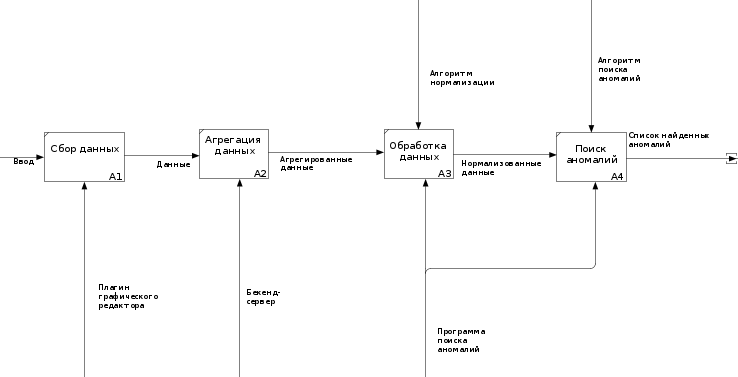
\includegraphics[width=.9\textwidth]{img2/idef0.png}
	\caption{Общая схема программного комплекса}
	\label{fig08}
\end{figure}
\section{Метод обнаружения аномалий}
На вход методу подается файл с нормализованными значениями атрибутов, с фиксированным заранее известным количеством атрибутов для каждого элемента. Временная отметка элемента представляется в качестве отдельного нормализованного атрибута. Допустимо отсуствие временной отметки.
Были выбраны методы: к-ближайших соседей,локальный коэффициент выбросов.
Каждый из вышеописанных методов инвариантен и иммутабелен относительно набора данных. В результате их работы получается три набора меток. На основе этих наборов формируется финвальный набор меток по следующему принципу: если элемент имеет две или более "аномальных" метки, то ему присвается "аномальная" метка, иначе - "нормальная" метка.
\section{Подбор параметров алгоритмов}
\subsection{Анализ резульатов работы методов}
\begin{figure}[!h]
	\centering
	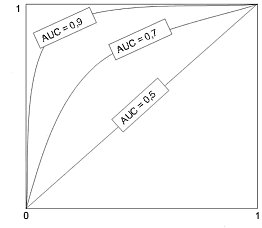
\includegraphics[width=.5\textwidth]{img/aucROc.png}
	\caption{Auc ROC}
	\label{fig06}
\end{figure}
Для проверки рабоспобности метода его нужно оценить при помощи наборов данных. Метрикой сравнения наборов данных был выбран AUC ROC — площадь под графиком, позволяющим оценить качество бинарной классификации, отображающим соотношение между долей объектов от общего количества носителей признака, верно классифицированных как несущих признак, и долей объектов от общего количества объектов, не несущих признака, ошибочно классифицированных как несущих признак. 

При помощи этой метрики планируется оценить адекватность работы алгоритма на размеченных наборах данных и  сравнить  с другими методами.
\subsection{Подбор параметров}
Алгоритмы поиска аномалий содержат некоторое различное количество параметров, которые необходимо указывать при работе алгоритмов. Однако, в отсутсвии априорной информации о данных, их необходимо подобрать, основываясь на валидирующем наборе данных. \cite{Book17}
Для этого будет использован простой генетический алгоритм.
Архитектура генетических алгоритмов позволяет найти решение быстрее за счет более 'осмысленного' перебора. Будет осуществляеться перебор не всего подряд, а приближаться от случайно выбранных решений к лучшим.
\begin{figure}
	\centering
	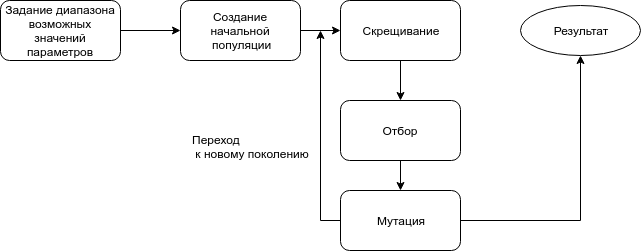
\includegraphics[width=.8\textwidth]{diagrams/diagram1.png}
	\caption{ Общий рисунок функционирования генетического алгоритма}
	\label{fig09}
\end{figure}
В качестве функции, для которой ищется экстремум, используется алгорит поиска аномалий, в качестве выходного значения функции - значение AUC ROC, полученное в результате работы алгоритма поиска аномалий на размеченном наборе данных. Критерием останова поиска оптимальных значений параметров алгоритма служит схождение популяции.
 Параметры, соответствующие наибольшему значению AUC ROC, сохраняются для использования в дальнейшем. 

\section{К ближайших соседей}
Метод основан на поиске аномальных значений расстояний до K ближайших соседей точки. Параметры алгоритма такие как K задаются после их нахождения вышеописанным методом.
\begin{lstlisting}[language=c++,,escapeinside={(@}{@)},caption={Алгоритм метода К ближайших соседей}] 
double calculateDist(vector<double> values, int orElen, int rInd, int lInt, int counter)
{
	while (counter) {
	int leftDistance = -1, rightDistance = -1;
	if (rightIndex > -1)
		rightDistance = abs(values[rightIndex]);
	if (leftIndex > -1)
		leftDistance = abs(values[leftIndex]);
	if (leftDistance > rightDistance) {
		rightIndex++;
		distance += abs(originalElement - rightDistance);
	} else {
		leftIndex++;
		distance += abs(originalElement - leftDistance);
	}
		counter--;
	}
}
double kNearestDistance(vector<double> values, double value, int k)
{
	int index = findIndex(values, value);
	double originalElement = values[index];
	double distance = 0;
	int rightIndex = index + 1, leftIndex = index - 1;
	int counter = k;

	return distance;
}

for (int i = 0; i < values.size(); i++) {
	for (int j = 0; j < values[i].size(); j++) {
		values[i][j].distance = kNearestDistance(sortedValues[j], values[i][j].value, dimensionSize, j);
		}
}
\end{lstlisting}
Псевдокод содержит часть алгоритма, которая позволяет определять дистанции между точками. Этот алгоритм отличается от классического алгоритма К ближайших соседей, тем что расстояние до K ближайших соседей находится не с помощью Евлкидова расстояния, а при помомощи разбиения исходного двумерного массива атрибутов на одномерные массивы атрибутов согласно классам атрибутов.

 Алгоритм нахождения расстояние для одного элемента:
 
\begin{enumerate}
	\item Для каждого атрибута находится k ближайших точек этого же класса
	\item Расстояние между искомым атрибутом и k ближайшими соседями суммируется
	\item Рассчитанные для каждого атрибута сумма складываются в итоговое расстояние
\end{enumerate}
Временная сложнось данного алгоритма O(n\^2), где n- суммарное количество атрибутов всех элементов данных. Сложность по памяти O(n).
\section{Локальный коэффициент выбросов}
\begin{lstlisting}[language=c++,,escapeinside={(@}{@)},caption={Алгоритм метода локального коэффициент выбросов}] 
auto calcLRD(vector<Point> values, Point value, int k, Mode mode)
{
	values.delete(value);
	vector<Point> nearPoints;
	
	for(i = 0; i < values.size(); ++i){
		if(distance(values[i], value) > k)
			nearPoints.pushback(value)
	}
	for(i = 0; i < nearPoints.size(); ++i){
		sum += nearPoints[i];
	}
	if(mode != sum)
		return nearPoints;
	else 
		return nearPoints.size()/sum;
}

double LOF(vector<Points> values, Point value,int k)
{
    vector<Point> nearPoints = caclLRD(values, value, k, val);
    int N = nearPoints.size()
    double lrdsSum = 0;
	for(int i=0; i < nearPoints.size(); ++i){
		lrds + = calcLRD(values, nearPoints[i],k), sum);
	}
	
	double result = lrdsSum/calcLrds(values, value,k, val);
	return result;		
}
vector<double> distances;
for (int i = 0; i < values.size(); i++) {
	distances.pushback(LOF(values,value,k)
}
\end{lstlisting}
Псевдокод содержит основные сущности алгоритма : нахождение LOF и LRD. Временная сложнось данного алгоритма O(n\^2), где n- суммарное количество атрибутов всех элементов данных. Сложность по памяти O(n).
\section{Компонентный коэффициент выбросов}
Алгоритм COF почти полностью повторяет алгоритм LOF, но отличается способом вычисления расстяния между двумя точками. Расстояние между двумя точками вычисляется при помощи метода "кратчайшей цепочки". Для всех  элементов набора данных строится матрица расстояний на основе евлидова расстояния.После этого при помощи алгоритма Флойда-Уоршела между двумя точками ищется кратчайший путь Длина этого кратчайшего пути и будет мерой расстояния между двумя точками. 

\begin{lstlisting}[language=c++,,escapeinside={(@}{@)},caption={Алгоритм Флойда — Уоршелла}] 
for k = 1 to n
	for i = 1 to n
		for j = 1 to n
			W[i][j] = min(W[i][j], W[i][k] + W[k][j])
\end{lstlisting}
\section{Собирающее данные для анализа ПО}
Для применения метода на практике было разработано ПО, которое позволяет собирать данные для анализа(телеметрию). В состав приложения будет входить плагин для графического редактора, backend-сервер, frontend. Так же на бекенде будет размещена база данных где будут размещаться необработанные данные.
 
\begin{figure}[h]
	\centering
	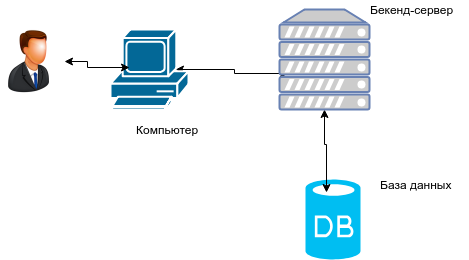
\includegraphics[width=.5\textwidth]{diagrams/diagram2.png}
	\caption{Общая архитектура приложения}\label{cha:design}
	\label{fig07}
\end{figure}
Результатом работы ПО будет неразмеченный набор данных, содержащий фиксированное количество атрибутов.
\subsection{Собираемые данные}
Основые собираемые данные приведены в таблице \ref{tab:collectdata}:

\begin{table}[!h]

\caption{\label{tab:collectdata}Описание собираемых данных}

\begin{center}

\begin{tabular}{|l|l|l|}

\hline

Информация о & Источник данных & Данные \\

\hline \hline

Инструменты & KisTool::activate, KisTool:deactivate & 

CountUse float64 

\tabularnewline & & Time     float64 

\tabularnewline & & ToolName string 

\tabularnewline & & Timestamp     float64 \\


\hline

Действия & 

KisMainWindows actioncollection()

& 

CountUse float64 

\tabularnewline & & TimeUse      float64 

\tabularnewline & & ActionName string 

\tabularnewline & & Timestamp     float64 \\


\hline

Cвойства изображений & 

KisDocument::saveFile()

& 

ColorProfile string 

\tabularnewline & &  ColorSpace   string 

\tabularnewline & & Height       float64 

\tabularnewline & & Width      float64

\tabularnewline & & Size      float64 

\tabularnewline & & NumLayers      float64 

\tabularnewline & & Timestamp     float64 \\


\hline


\end{tabular}

\end{center}

\end{table}
\subsection{Клиентская часть}
Был разработан плагин для графического редактора Krita, который позво­
ляет собирать телеметрию с пользователей. Телеметрия собирается только во время работы программы и при закрытия программы собранные данные удаляются с компьютера пользователя.Телеметрия отправляется через опре­деленные интервалы времени на удаленный серве. Записи о действиях и инстру­ментах отправляются каждые n минут.	   Информация о свойствах иозбражения собирается при сохранения изображения. 


Собираемые метрики агрегруются на стороне клиента в http-запрос. Пример тела запроса представляет собою JSON, пример этого JSON приведен ниже(форматирование нарушено в целях наглядности).
\begin{lstlisting}[language=c++,,escapeinside={(@}{@)},caption={Тело http-запроса}] 
{
"Name": [
{
"Param1": 1,
"Param2": 4581,
"Timestamp": 12214
},
\end{lstlisting}
\subsection{Серверная часть}
На сервере метрики обработываются и заносятся в базу данных в формате JSON. Сервер способен принимать и обрабатывать много параллельных запросов пользователей.
Наличие временной отметки  у элементов данных позволяет извлекать данные за определенный промежуток времени.
	\begin{lstlisting}[language=c++,,escapeinside={(@}{@)},caption={Пример хранимого элемента в базе данных}] 
	{ "\_id" : ObjectId("5b08a54677d37ee1964df0b7"), "actions" : [ { "countuse" : 1, "sources" : 0, "actionname" : "edit\_cut", "time" : 1527293254 }
	\end{lstlisting}

\subsection{Динамическое изменение данных}
Инструменты и действия(actions) могут меняться достаточно часто в про­цессе разработки графическего редактора. Поэтому неразумно задавать статически
эти метрики в коде. В коде бекенд-сервера реализована поддержка добавления но­вых элементов. Раз в сутки просыпается новая горутина(легковесный тред), которая пробегается по базе данных и ищет новые инструменты и действия. После этого она записывает их в текстовый файл. Подобное разумно применять не только для инструментов и действий, но и для любых часто изменяющихся данных.  В будущем возможно расширения этой системы.